% answers.tex —— 2007 年·全国大纲卷Ⅰ·理科 · 参考答案与详细解析片段
% 由 tools/generate_projects.py 依来源总账自 2007/2007_数学真题_全国1理_试题.md + 2007/2007_数学真题_全国1理_解析正文.md + 2007/2007_数学真题_全国1理_答案要点.md 生成，勿手改（改源 MD 后重跑）


\begin{gktip}
固定源 PDF 为印刷页码 359–360 的两页题面，不附答案。以下解析均依据固定源独立复算；第 7、19 题图形在 LaTeX 工程中以 TikZ/PGFPlots 矢量源重绘。
\end{gktip}

\begin{answer}
\gksolhead{1}{}

\textbf{题目}：

$\alpha$ 是第四象限角，$\tan\alpha=-\dfrac5{12}$，则 $\sin\alpha=$\mbox{（　　）}

（A）$\dfrac15$\quad（B）$-\dfrac15$\quad（C）$\dfrac5{13}$\quad（D）$-\dfrac5{13}$

\Needspace{4\baselineskip}
\textbf{解析}

第四象限内 $\cos\alpha>0,\sin\alpha<0$，由 $\tan\alpha=-5/12$ 得 $\sin\alpha=-5/13$。

\gkanswer{答案：D}

\end{answer}
\begin{answer}
\gksolhead{2}{}

\textbf{题目}：

设 $a$ 是实数，且 $\dfrac{a}{1+i}+\dfrac{1+i}{2}$ 是实数，则 $a=$\mbox{（　　）}

（A）$\dfrac12$\quad（B）$1$\quad（C）$\dfrac32$\quad（D）$2$

\Needspace{4\baselineskip}
\textbf{解析}

\nopagebreak[4]
\[
\frac{a}{1+i}+\frac{1+i}{2}
=\frac{a(1-i)}2+\frac{1+i}{2}
\]
，

虚部为零给出 $a=1$。

\gkanswer{答案：B}

\end{answer}
\begin{answer}
\gksolhead{3}{}

\textbf{题目}：

已知向量 $\boldsymbol a=(-5,6)$，$\boldsymbol b=(6,5)$，则 $\boldsymbol a$ 与 $\boldsymbol b$\mbox{（　　）}

（A）垂直\quad（B）不垂直也不平行\quad（C）平行且同向\quad（D）平行且反向

\Needspace{4\baselineskip}
\textbf{解析}

\nopagebreak[4]
\[
\boldsymbol a\cdot\boldsymbol b=(-5)6+6\cdot5=0
\]
。

\gkanswer{答案：A}

\end{answer}
\begin{answer}
\gksolhead{4}{}

\textbf{题目}：

已知双曲线的离心率为 $2$，焦点是 $(-4,0),(4,0)$，则双曲线方程为\mbox{（　　）}

（A）$\dfrac{x^2}{4}-\dfrac{y^2}{12}=1$\quad（B）$\dfrac{x^2}{12}-\dfrac{y^2}{4}=1$\quad（C）$\dfrac{x^2}{10}-\dfrac{y^2}{6}=1$\quad（D）$\dfrac{x^2}{6}-\dfrac{y^2}{10}=1$

\Needspace{4\baselineskip}
\textbf{解析}

与全国卷Ⅰ文科第 4 题相同，$c=4,e=2$，故 $a=2,b^2=12$，方程为 $x^2/4-y^2/12=1$。

\gkanswer{答案：A}

\end{answer}
\begin{answer}
\gksolhead{5}{}

\textbf{题目}：

设 $a,b\in\mathbb R$，集合 $\{1,a+b,a\}=\left\{0,\dfrac ba,b\right\}$，则 $b-a=$\mbox{（　　）}

（A）$1$\quad（B）$-1$\quad（C）$2$\quad（D）$-2$

\Needspace{4\baselineskip}
\textbf{解析}

集合右侧含 $0$，而 $a\ne0$，故左侧只能由 $a+b=0$ 产生 $0$。于是 $b=-a$，再比较两个三元集合可得 $a=-1,b=1$，所以 $b-a=2$。

\gkanswer{答案：C}

\end{answer}
\begin{answer}
\gksolhead{6}{}

\textbf{题目}：

\Needspace{5\baselineskip}
下面给出的四个点中，到直线 $x-y+1=0$ 的距离为 $\dfrac{\sqrt2}{2}$，且位于不等式组

\nopagebreak[4]
\[
\begin{cases}
x+y-1<0,\\
x-y+1>0
\end{cases}
\]

表示的平面区域内的点是\mbox{（　　）}

（A）$(1,1)$\quad（B）$(-1,1)$\quad（C）$(-1,-1)$\quad（D）$(1,-1)$

\Needspace{4\baselineskip}
\textbf{解析}

距离条件给出 $|x-y+1|=1$。逐点检验不等式组后，只有 $(-1,-1)$ 满足。

\gkanswer{答案：C}

\end{answer}
\begin{answer}
\gksolhead{7}{}

\textbf{题目}：

如图，正四棱柱 $ABCD-A_1B_1C_1D_1$ 中，$AA_1=2AB$，则异面直线 $A_1B$ 与 $AD_1$ 所成角的余弦值为\mbox{（　　）}
\nopagebreak[4]
\begin{center}% 2007 年全国大纲卷Ⅰ理科第 7 题：正四棱柱
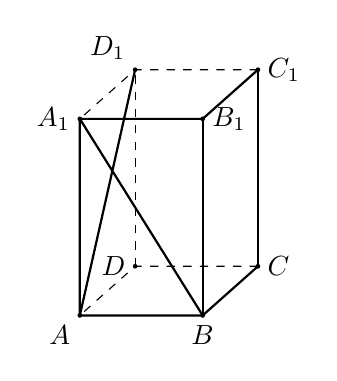
\begin{tikzpicture}[>=stealth,scale=0.78]
  \coordinate (A) at (0,0); \coordinate (B) at (2.0,0);
  \coordinate (C) at (2.9,0.8); \coordinate (D) at (0.9,0.8);
  \coordinate (A1) at (0,3.2); \coordinate (B1) at (2,3.2);
  \coordinate (C1) at (2.9,4.0); \coordinate (D1) at (0.9,4.0);
  \draw[thick] (A)--(B)--(C); \draw[dashed] (C)--(D)--(A);
  \draw[thick] (A)--(A1)--(B1)--(C1);
  \draw[dashed] (C1)--(D1)--(A1);
  \draw[thick] (B)--(B1) (C)--(C1);
  \draw[dashed] (D)--(D1);
  \draw[thick] (A1)--(B) (A)--(D1);
  \fill (A) circle (1.1pt) node[below left] {$A$};
  \fill (B) circle (1.1pt) node[below] {$B$};
  \fill (C) circle (1.1pt) node[right] {$C$};
  \fill (D) circle (1.1pt) node[left] {$D$};
  \fill (A1) circle (1.1pt) node[left] {$A_1$};
  \fill (B1) circle (1.1pt) node[right] {$B_1$};
  \fill (C1) circle (1.1pt) node[right] {$C_1$};
  \fill (D1) circle (1.1pt) node[above left] {$D_1$};
\end{tikzpicture}
\end{center}
\nopagebreak[4]
（A）$\dfrac15$\quad（B）$\dfrac25$\quad（C）$\dfrac35$\quad（D）$\dfrac45$

\Needspace{4\baselineskip}
\textbf{解析}

与全国卷Ⅰ文科第 7 题相同，取棱长 $AB=1,AA_1=2$，得到两方向向量的夹角余弦为 $4/5$。

\gkanswer{答案：D}

\end{answer}
\begin{answer}
\gksolhead{8}{}

\textbf{题目}：

设 $a>1$，函数 $f(x)=\log_a x$ 在区间 $[a,2a]$ 上的最大值与最小值之差为 $\dfrac12$，则 $a=$\mbox{（　　）}

（A）$\sqrt2$\quad（B）$2$\quad（C）$2\sqrt2$\quad（D）$4$

\Needspace{4\baselineskip}
\textbf{解析}

对数函数在 $[a,2a]$ 上递增，故差值为 $\log_a2=1/2$，得到 $a=4$。

\gkanswer{答案：D}

\end{answer}
\begin{answer}
\gksolhead{9}{}

\textbf{题目}：

$f(x),g(x)$ 是定义在 $\mathbb R$ 上的函数，$h(x)=f(x)+g(x)$，则“$f(x),g(x)$ 均为偶函数”是“$h(x)$ 为偶函数”的\mbox{（　　）}

（A）充要条件\quad（B）充分而不必要的条件\quad（C）必要而不充分的条件\quad（D）既不充分也不必要的条件

\Needspace{4\baselineskip}
\textbf{解析}

偶函数相加仍为偶函数，但和为偶函数不能推出两个加数分别为偶函数，例如 $f(x)=x,g(x)=-x$。故选充分而不必要。

\gkanswer{答案：B}

\end{answer}
\begin{answer}
\gksolhead{10}{}

\textbf{题目}：

在 $\left(x^2-\dfrac1x\right)^n$ 的展开式中，常数项为 $15$，则 $n=$\mbox{（　　）}

（A）$3$\quad（B）$4$\quad（C）$5$\quad（D）$6$

\Needspace{4\baselineskip}
\textbf{解析}

常数项要求 $2n-3k=0$，系数为 $\binom nk(-1)^k=15$。取 $k=2$ 得 $n=6$，满足条件。

\gkanswer{答案：D}

\end{answer}
\begin{answer}
\gksolhead{11}{}

\textbf{题目}：

抛物线 $y^2=4x$ 的焦点为 $F$，准线为 $l$，经过 $F$ 且斜率为 $\sqrt3$ 的直线与抛物线在 $x$ 轴上方的部分相交于点 $A$，$AK\perp l$，垂足为 $K$，且 $\triangle AKF$ 的面积是\mbox{（　　）}

（A）$4$\quad（B）$3\sqrt3$\quad（C）$4\sqrt3$\quad（D）$8$

\Needspace{4\baselineskip}
\textbf{解析}

与全国卷Ⅰ文科第 12 题相同，交点为 $(3,2\sqrt3)$，三角形面积为 $4\sqrt3$。

\gkanswer{答案：C}

\end{answer}
\begin{answer}
\gksolhead{12}{}

\textbf{题目}：

函数 $f(x)=\cos^2x-2\cos^2\dfrac x2$ 的一个单调增区间是\mbox{（　　）}

（A）$\left(\dfrac\pi3,\dfrac{2\pi}3\right)$\quad（B）$\left(\dfrac\pi6,\dfrac\pi2\right)$\quad（C）$\left(0,\dfrac\pi3\right)$\quad（D）$\left(-\dfrac\pi6,\dfrac\pi6\right)$

\Needspace{4\baselineskip}
\textbf{解析}

\nopagebreak[4]
\[
f'(x)=-\sin2x+\sin x=\sin x(1-2\cos x)
\]
。

在 $(\pi/3,2\pi/3)$ 内导数为正，故该区间为单调增区间。

\gkanswer{答案：A}

\end{answer}
\begin{answer}
\gksolhead{13}{}

\textbf{题目}：

从班委会 $5$ 名成员中选出 $3$ 名，分别担任班级学习委员、文娱委员与体育委员，其中甲、乙二人不能担任文娱委员，则不同的选法共有\gkblank{}种。（用数字作答）

\Needspace{4\baselineskip}
\textbf{解析}

文娱委员有 $3$ 种选择，另外两个职位从剩下 $4$ 人中有 $4\times3$ 种安排，共 $36$ 种。

\gkanswer{答案：$36$}

\end{answer}
\begin{answer}
\gksolhead{14}{}

\textbf{题目}：

函数 $y=f(x)$ 的图象与函数 $y=\log_3x\ (x>0)$ 的图象关于直线 $y=x$ 对称，则 $f(x)=$\gkblank{}。

\Needspace{4\baselineskip}
\textbf{解析}

反函数关系给出 $f(x)=3^x$。

\gkanswer{答案：$3^x$}

\end{answer}
\begin{answer}
\gksolhead{15}{}

\textbf{题目}：

等比数列 $\{a_n\}$ 的前 $n$ 项和 $S_n$，已知 $S_1,2S_2,3S_3$ 成等差数列，则 $\{a_n\}$ 的公比为\gkblank{}。

\Needspace{4\baselineskip}
\textbf{解析}

由 $S_1+3S_3=4S_2$ 得 $q(3q-1)=0$。等比数列公比非零，故 $q=1/3$。

\gkanswer{答案：$\dfrac13$}

\end{answer}
\begin{answer}
\gksolhead{16}{}

\textbf{题目}：

一个等腰直角三角形的三个顶点分别在正三棱柱的三条侧棱上。已知正三棱柱的底面边长为 $2$，则该三角形的斜边长为\gkblank{}。

\Needspace{4\baselineskip}
\textbf{解析}

\Needspace{5\baselineskip}
设三个侧棱上的点相对同一顶点的高度差为 $u,v$。底面水平距离均为 $2$。直角等腰条件给出 $u^2=v^2=2$，两直角边端点间的距离满足

\nopagebreak[4]
\[
c^2=2^2+(2\sqrt2)^2=12
\]
，

故斜边长为 $2\sqrt3$。

\gkanswer{答案：$2\sqrt3$}

\end{answer}
\begin{answer}
\gksolhead{17}{}

\textbf{题目}：

设锐角三角形 $ABC$ 的内角 $A,B,C$ 的对边分别为 $a,b,c$，$a=2b\sin A$。

（1） 求 $B$ 的大小；

（2） 求 $\cos A+\sin C$ 的取值范围。

\Needspace{4\baselineskip}
\textbf{解析}

\gksubpart{(1)}

正弦定理将 $a=2b\sin A$ 化为 $\sin B=1/2$，锐角条件给出 $B=\pi/6$。

\gksubpart{(2)}

\Needspace{5\baselineskip}
此时 $A+C=5\pi/6$，令 $A\in(\pi/3,\pi/2)$，则

\nopagebreak[4]
\[
\cos A+\sin C
=\cos A+\sin\left(\frac{5\pi}{6}-A\right)
=\frac32\cos A+\frac{\sqrt3}{2}\sin A
\]
。

该函数在上述开区间递减，故值域为 $\left(\dfrac{\sqrt3}{2},\dfrac32\right)$。

\gkanswer{答案（1）：$B=\dfrac\pi6$。}

\gkanswer{答案（2）：$\dfrac{\sqrt3}{2}<\cos A+\sin C<\dfrac32$。}

\end{answer}
\begin{answer}
\gksolhead{18}{}

\textbf{题目}：

某商场经销某商品，根据以往资料统计，顾客采用的付款期为随机变量 $\xi$ 的分布列为

\begin{center}
\begin{tabular}{lrrrrr}
\toprule
$\xi$ & $1$ & $2$ & $3$ & $4$ & $5$ \\
\midrule
$P$ & $0.4$ & $0.2$ & $0.2$ & $0.1$ & $0.1$ \\
\bottomrule
\end{tabular}
\end{center}

商场经销一件该商品，采用 $1$ 期付款，基利润为 $200$ 元；分 $2$ 期或 $3$ 期付款，基利润为 $250$ 元；分 $4$ 期或 $5$ 期付款，其利润为 $300$ 元。$\eta$ 表示经销一件该商品的利润。

（1） 求事件 $A$：“购买该商品的 $3$ 位顾客中，至少有 $1$ 位采用 $1$ 期付款”的概率 $P(A)$；

（2） 求 $\eta$ 的分布列及期望 $E\eta$。

\Needspace{4\baselineskip}
\textbf{解析}

\gksubpart{(1)}

三位顾客均不采用 $1$ 期付款的概率为 $0.6^3$，所以 $P(A)=1-0.6^3=0.784$。

\gksubpart{(2)}

\Needspace{5\baselineskip}
利润 $\eta$ 取 $200,250,300$ 的概率分别为 $0.4,0.4,0.2$，且

\nopagebreak[4]
\[
E\eta=200(0.4)+250(0.4)+300(0.2)=240
\]
。

\gkanswer{答案（1）：$P(A)=0.784$。}

\gkanswer{答案（2）：$P(\eta=200)=0.4$，$P(\eta=250)=0.4$，$P(\eta=300)=0.2$；$E\eta=240$。}

\end{answer}
\begin{answer}
\gksolhead{19}{}

\textbf{题目}：

四棱锥 $S-ABCD$ 中，底面 $ABCD$ 为平行四边形，侧面 $SBC\perp$ 底面 $ABCD$。已知 $\angle ABC=45^\circ$，$AB=2$，$BC=2\sqrt2$，$SA=SB=\sqrt3$。
\nopagebreak[4]
\begin{center}% 2007 年全国大纲卷Ⅰ理科第 19 题：四棱锥
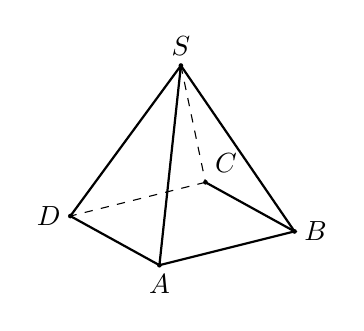
\begin{tikzpicture}[>=stealth,scale=0.78]
  \coordinate (A) at (1.8,0); \coordinate (B) at (4.0,0.55);
  \coordinate (C) at (2.55,1.35); \coordinate (D) at (0.35,0.8);
  \coordinate (S) at (2.15,3.25);
  \draw[thick] (A)--(B)--(C); \draw[dashed] (C)--(D); \draw[thick] (D)--(A);
  \draw[thick] (S)--(A) (S)--(B) (S)--(D);
  \draw[dashed] (S)--(C);
  \fill (S) circle (1.1pt) node[above] {$S$};
  \fill (A) circle (1.1pt) node[below] {$A$};
  \fill (B) circle (1.1pt) node[right] {$B$};
  \fill (C) circle (1.1pt) node[above right] {$C$};
  \fill (D) circle (1.1pt) node[left] {$D$};
\end{tikzpicture}
\end{center}
\nopagebreak[4]
（1） 证明：$SA\perp BC$；

（2） 求直线 $SD$ 与平面 $SAB$ 所成角的大小。

\Needspace{4\baselineskip}
\textbf{解析}

\gksubpart{(1)}

坐标化方式与全国卷Ⅰ文科第 19 题相同，直接得到 $SA\perp BC$。

\gksubpart{(2)}

\Needspace{5\baselineskip}
由 $SA=SB=\sqrt3$ 得 $S=(\sqrt2,0,1)$（取适当坐标系），计算平面法向量与 $SD$ 的夹角，得到

\nopagebreak[4]
\[
\sin\theta=\sqrt{\frac2{11}},
\qquad \cos\theta=\frac3{\sqrt{11}}
\]
。

\gkanswer{答案（1）：见解析版}

\gkanswer{答案（2）：$\cos\theta=\dfrac3{\sqrt{11}}$。}

\end{answer}
\begin{answer}
\gksolhead{20}{}

\textbf{题目}：

设函数 $f(x)=e^x-e^{-x}$。

（1） 证明：$f(x)$ 的导数 $f'(x)\geqslant2$；

（2） 若对所有 $x\geqslant0$ 都有 $f(x)\geqslant ax$，求 $a$ 的取值范围。

\Needspace{4\baselineskip}
\textbf{解析}

\gksubpart{(1)}

\nopagebreak[4]
\[
f'(x)=e^x+e^{-x}\geqslant2
\]

由基本不等式成立。

\gksubpart{(2)}

对 $x\geqslant0$ 积分得 $f(x)-f(0)\geqslant2x$，即 $f(x)\geqslant2x$。又 $x\to0^+$ 时 $f(x)/x\to2$，故充要条件为 $a\leqslant2$。

\gkanswer{答案（1）：$a\leqslant2$。}

\gkanswer{答案（2）：见解析版}

\end{answer}
\begin{answer}
\gksolhead{21}{}

\textbf{题目}：

已知椭圆 $\dfrac{x^2}{3}+\dfrac{y^2}{2}=1$ 的左、右焦点分别为 $F_1,F_2$，过 $F_1$ 的直线交椭圆于 $B,D$ 两点，过 $F_2$ 的直线交椭圆于 $A,C$ 两点，且 $AC\perp BD$，垂足为 $P$。

（1） 设 $P$ 点的坐标为 $(x_0,y_0)$，证明：$\dfrac{x_0^2}{3}+\dfrac{y_0^2}{2}<1$；

（2） 求四边形 $ABCD$ 的面积的最小值。

\Needspace{4\baselineskip}
\textbf{解析}

\gksubpart{(1)}

\Needspace{5\baselineskip}
两条互相垂直的椭圆弦交于椭圆内部点，严格凸性给出

\nopagebreak[4]
\[
\frac{x_0^2}{3}+\frac{y_0^2}{2}<1
\]
。

\gksubpart{(2)}

\Needspace{5\baselineskip}
设过右焦点弦方向角为 $t$，两条垂直弦的长度分别为

\nopagebreak[4]
\[
\frac{4\sqrt3}{2\cos^2t+3\sin^2t},
\qquad
\frac{4\sqrt3}{2\sin^2t+3\cos^2t}
\]
。

四边形面积为两对角线乘积的一半，化简后分母最大为 $25/4$，故最小面积为 $96/25$。

\gkanswer{答案（1）：见解析版}

\gkanswer{答案（2）：四边形面积最小值为 $\dfrac{96}{25}$。}

\end{answer}
\begin{answer}
\gksolhead{22}{}

\textbf{题目}：

已知数列 $\{a_n\}$ 中 $a_1=2$，$a_{n+1}=(\sqrt2-1)(a_n+2)$，$n=1,2,3,\ldots$。

（1） 求 $\{a_n\}$ 的通项公式；

（2） 若数列 $\{b_n\}$ 中 $b_1=2$，$b_{n+1}=\dfrac{3b_n+4}{2b_n+3}$，$n=1,2,3,\ldots$，证明：$b_n<b_{n+1}$，其中 $n$ 为正整数。

\Needspace{4\baselineskip}
\textbf{解析}

\gksubpart{(1)}

\Needspace{5\baselineskip}
递推式的平衡点为 $\sqrt2$，所以

\nopagebreak[4]
\[
a_n=\sqrt2+(2-\sqrt2)(\sqrt2-1)^{n-1}
\]
。

\gksubpart{(2)}

\Needspace{5\baselineskip}
令 $\phi(t)=t^2(3-2t)$，则 $b_n^2=\phi(a_n)$，并且

\nopagebreak[4]
\[
\phi\left(\frac{3-t}{2}\right)-\phi(t)
=\frac94t(t-1)^2>0
\]

对所有 $a_n\in(0,3/2)$ 且 $a_n\ne1$ 成立，故 $b_n<b_{n+1}$。

\gkanswer{答案（1）：$a_n=\sqrt2+(2-\sqrt2)(\sqrt2-1)^{n-1}$。}

\gkanswer{答案（2）：见解析版}

\end{answer}